\documentclass{article}
\usepackage{graphicx} % Required for inserting images
\usepackage{longtable}

\title{Assignment 2}
\author{Claire Zhang}
\date{November 4, 2023}

\begin{document}

\maketitle

\section{Difference-in-Differences Line Graph}
\begin{figure}[htbp]

\caption{\textbf{Average Lung Hospitalizations over Time}
\label{tab:EngApproach}}
\center
	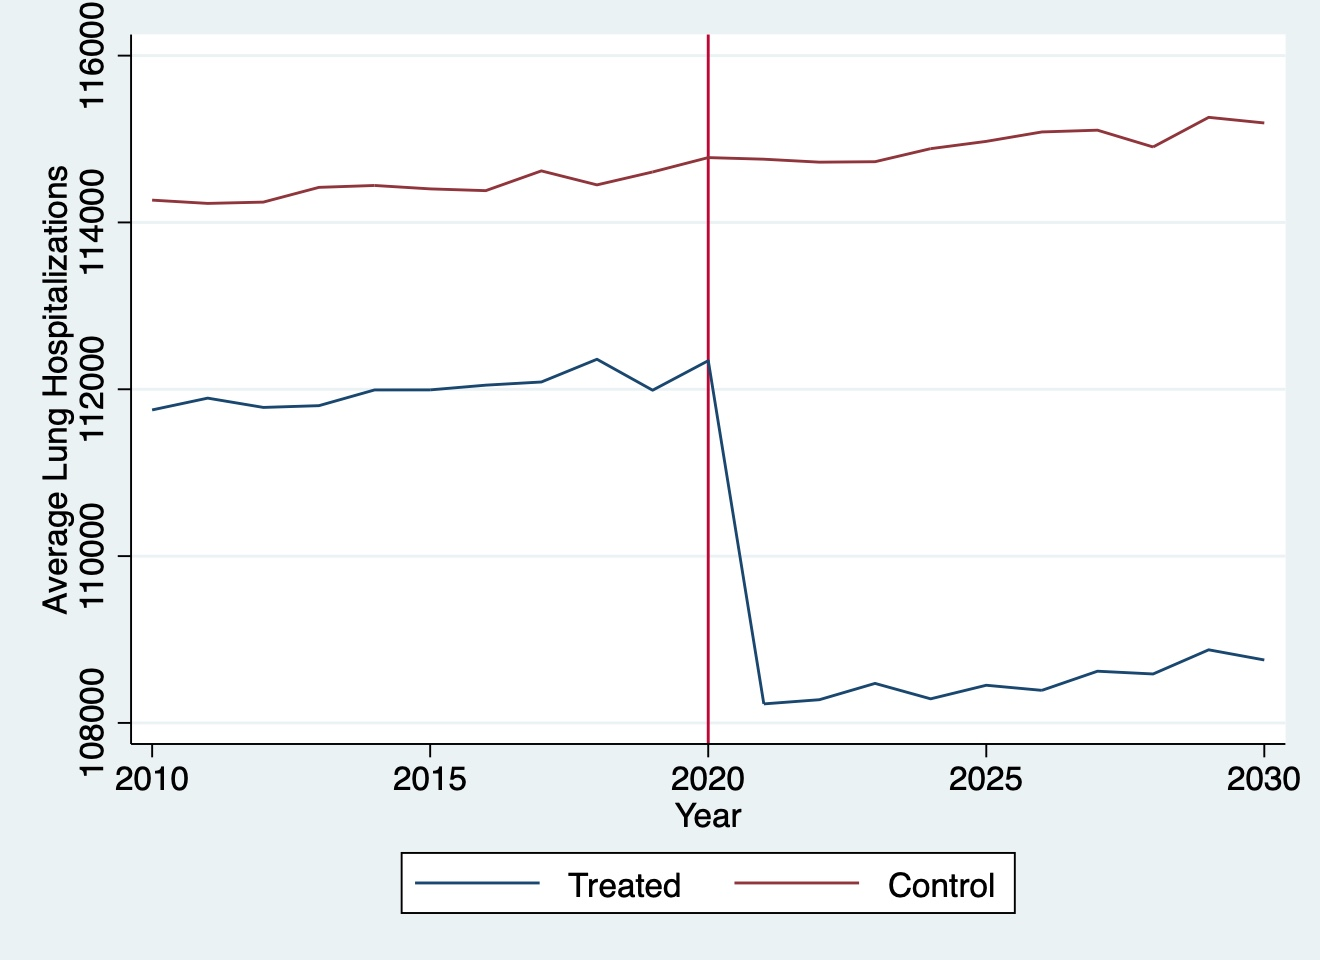
\includegraphics[width=90mm]{didlinegraph.jpg}
    \center
    \begin{footnotesize}
    \textbf Prior to the vaping bans going into effect in 2021, we see that the trend lines for the treated and control states have similar trends. However, after 2020, the average number of lung hospitalizations across treated states appear to be much smaller than those in the control states.  
    \end{footnotesize}
\end{figure}
\newpage

\section{Regression Tables}

{
\def\sym#1{\ifmmode^{#1}\else\(^{#1}\)\fi}
\begin{longtable}{l*{2}{c}}
\hline\hline\endfirsthead\hline\endhead\hline\endfoot\endlastfoot
                    &\multicolumn{1}{c}{(1)}&\multicolumn{1}{c}{(2)}\\
                    &\multicolumn{1}{c}{Parallel Trends Test}&\multicolumn{1}{c}{DiD}\\
\hline
treated\_year        &      -1.209\sym{***}&                     \\
                    &    (-31.46)         &                     \\
[1em]
treated\_post        &                     &     -4030.5\sym{***}\\
                    &                     &    (-61.64)         \\
[1em]
State=1             &                     &           0         \\
                    &                     &         (.)         \\
[1em]
State=2             &                     &      -203.4         \\
                    &                     &     (-1.25)         \\
[1em]
State=3             &                     &       229.3         \\
                    &                     &      (1.41)         \\
[1em]
State=4             &                     &       54.38         \\
                    &                     &      (0.33)         \\
[1em]
State=5             &                     &       483.8\sym{**} \\
                    &                     &      (2.97)         \\
[1em]
State=6             &                     &       411.7\sym{*}  \\
                    &                     &      (2.53)         \\
[1em]
State=7             &                     &       464.7\sym{**} \\
                    &                     &      (2.86)         \\
[1em]
State=8             &                     &       453.9\sym{**} \\
                    &                     &      (2.79)         \\
[1em]
State=9             &                     &       971.4\sym{***}\\
                    &                     &      (5.97)         \\
[1em]
State=10            &                     &       632.8\sym{***}\\
                    &                     &      (3.89)         \\
[1em]
State=11            &                     &       969.6\sym{***}\\
                    &                     &      (5.96)         \\
[1em]
State=12            &                     &      1002.0\sym{***}\\
                    &                     &      (6.16)         \\
[1em]
State=13            &                     &      1092.6\sym{***}\\
                    &                     &      (6.71)         \\
[1em]
State=14            &                     &      1225.7\sym{***}\\
                    &                     &      (7.53)         \\
[1em]
State=15            &                     &      1360.2\sym{***}\\
                    &                     &      (8.36)         \\
[1em]
State=16            &                     &      1257.0\sym{***}\\
                    &                     &      (7.72)         \\
[1em]
State=17            &                     &      1482.4\sym{***}\\
                    &                     &      (9.11)         \\
[1em]
State=18            &                     &      1819.9\sym{***}\\
                    &                     &     (11.18)         \\
[1em]
State=19            &                     &      1598.8\sym{***}\\
                    &                     &      (9.82)         \\
[1em]
State=20            &                     &      1774.2\sym{***}\\
                    &                     &     (10.90)         \\
[1em]
State=21            &                     &      2078.9\sym{***}\\
                    &                     &     (12.77)         \\
[1em]
State=22            &                     &      1995.4\sym{***}\\
                    &                     &     (12.26)         \\
[1em]
State=23            &                     &      2030.8\sym{***}\\
                    &                     &     (12.48)         \\
[1em]
State=24            &                     &      1979.1\sym{***}\\
                    &                     &     (11.94)         \\
[1em]
State=25            &                     &      2182.9\sym{***}\\
                    &                     &     (13.17)         \\
[1em]
State=26            &                     &      2266.3\sym{***}\\
                    &                     &     (13.68)         \\
[1em]
State=27            &                     &      2458.9\sym{***}\\
                    &                     &     (14.84)         \\
[1em]
State=28            &                     &      2535.4\sym{***}\\
                    &                     &     (15.30)         \\
[1em]
State=29            &                     &      2627.4\sym{***}\\
                    &                     &     (15.86)         \\
[1em]
State=30            &                     &      2738.8\sym{***}\\
                    &                     &     (16.53)         \\
[1em]
State=31            &                     &      2923.4\sym{***}\\
                    &                     &     (17.64)         \\
[1em]
State=32            &                     &      3128.3\sym{***}\\
                    &                     &     (18.88)         \\
[1em]
State=33            &                     &      3099.8\sym{***}\\
                    &                     &     (18.71)         \\
[1em]
State=34            &                     &      3120.5\sym{***}\\
                    &                     &     (18.83)         \\
[1em]
State=35            &                     &      3223.7\sym{***}\\
                    &                     &     (19.46)         \\
[1em]
State=36            &                     &      3288.3\sym{***}\\
                    &                     &     (19.84)         \\
[1em]
State=37            &                     &      3433.5\sym{***}\\
                    &                     &     (20.72)         \\
[1em]
State=38            &                     &      3462.1\sym{***}\\
                    &                     &     (20.89)         \\
[1em]
State=39            &                     &      3748.6\sym{***}\\
                    &                     &     (22.62)         \\
[1em]
State=40            &                     &      3809.3\sym{***}\\
                    &                     &     (22.99)         \\
[1em]
State=41            &                     &      3823.5\sym{***}\\
                    &                     &     (23.08)         \\
[1em]
State=42            &                     &      3960.6\sym{***}\\
                    &                     &     (23.90)         \\
[1em]
State=43            &                     &      3993.4\sym{***}\\
                    &                     &     (24.10)         \\
[1em]
State=44            &                     &      3996.4\sym{***}\\
                    &                     &     (24.12)         \\
[1em]
State=45            &                     &      4161.8\sym{***}\\
                    &                     &     (25.12)         \\
[1em]
State=46            &                     &      4389.1\sym{***}\\
                    &                     &     (26.49)         \\
[1em]
State=47            &                     &      4584.8\sym{***}\\
                    &                     &     (27.67)         \\
[1em]
State=48            &                     &      4624.6\sym{***}\\
                    &                     &     (27.91)         \\
[1em]
State=49            &                     &      4504.9\sym{***}\\
                    &                     &     (27.19)         \\
[1em]
State=50            &                     &      4917.5\sym{***}\\
                    &                     &     (29.68)         \\
[1em]
Year=2010           &                     &           0         \\
                    &                     &         (.)         \\
[1em]
Year=2011           &                     &       43.72         \\
                    &                     &      (0.41)         \\
[1em]
Year=2012           &                     &       1.140         \\
                    &                     &      (0.01)         \\
[1em]
Year=2013           &                     &       106.0         \\
                    &                     &      (1.01)         \\
[1em]
Year=2014           &                     &       205.0         \\
                    &                     &      (1.94)         \\
[1em]
Year=2015           &                     &       183.3         \\
                    &                     &      (1.74)         \\
[1em]
Year=2016           &                     &       198.0         \\
                    &                     &      (1.88)         \\
[1em]
Year=2017           &                     &       343.4\sym{**} \\
                    &                     &      (3.26)         \\
[1em]
Year=2018           &                     &       378.0\sym{***}\\
                    &                     &      (3.58)         \\
[1em]
Year=2019           &                     &       291.1\sym{**} \\
                    &                     &      (2.76)         \\
[1em]
Year=2020           &                     &       546.8\sym{***}\\
                    &                     &      (5.18)         \\
[1em]
Year=2021           &                     &       497.9\sym{***}\\
                    &                     &      (4.54)         \\
[1em]
Year=2022           &                     &       502.0\sym{***}\\
                    &                     &      (4.58)         \\
[1em]
Year=2023           &                     &       594.6\sym{***}\\
                    &                     &      (5.42)         \\
[1em]
Year=2024           &                     &       593.9\sym{***}\\
                    &                     &      (5.41)         \\
[1em]
Year=2025           &                     &       716.2\sym{***}\\
                    &                     &      (6.53)         \\
[1em]
Year=2026           &                     &       748.9\sym{***}\\
                    &                     &      (6.83)         \\
[1em]
Year=2027           &                     &       865.8\sym{***}\\
                    &                     &      (7.89)         \\
[1em]
Year=2028           &                     &       742.0\sym{***}\\
                    &                     &      (6.76)         \\
[1em]
Year=2029           &                     &      1067.1\sym{***}\\
                    &                     &      (9.73)         \\
[1em]
Year=2030           &                     &       974.6\sym{***}\\
                    &                     &      (8.89)         \\
[1em]
Constant            &    114439.8\sym{***}&    110787.4\sym{***}\\
                    &   (2180.10)         &    (807.50)         \\
\hline
Observations        &         550         &        1050         \\
\hline\hline
\multicolumn{3}{l}{\footnotesize \textit{t} statistics in parentheses}\\
\multicolumn{3}{l}{\footnotesize \sym{*} \(p<0.05\), \sym{**} \(p<0.01\), \sym{***} \(p<0.001\)}\\
\end{longtable}
}

\newpage
\section{Questions}

\textit{How many state-level fixed effects are there?} \\

There are 50 state-level fixed effects.\\
\\
\textit{What is the interpretation of the coefficient for each state-level fixed effect?} \\

The coefficient for each state-level fixed effect is not zero, relative to state 1. The coefficients are significant for all states except for 3. This would mean that there variation between states when it comes to lung hospitalization.\\
\\
\textit{Can you reject the hypothesis that state fixed effects are all zero?} \\

With the \textit{testparm} function, we test whether state ID fixed effects are equal to zero. Since the p-value is 0.0000, we reject the null hypothesis that the state fixed effects are zero.


\end{document}
